%\documentclass{standalone}
%\usepackage{amsmath}
%\usepackage{tikz}
%\usepackage{xcolor}
%\usetikzlibrary{fit,positioning}
%\begin{document}

% ---------------------------------------------------
% Comment above for inclusion in other docs
% ---------------------------------------------------


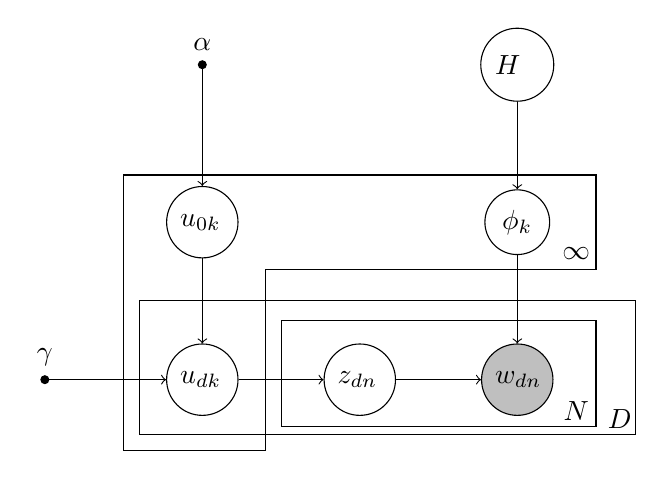
\begin{tikzpicture}

\coordinate (alpha_zero)   at (0,2);
\node (alpha_zero) at (2,4) [circle, draw, inner sep=1pt, fill, label=above:$\alpha$] { };
\node (theta_zero) at (2,2) [circle, draw, text width = 16pt] {$\text{ }u_{0k}$};

\coordinate (alpha)   at (0,0);
\node (alpha) at (0,0) [circle, draw, inner sep=1pt, fill, label=above:$\gamma$] { };
\node (theta) at (2,0) [circle, draw, text width = 16pt] {$\text{ }u_{dk}$};

\node (b) at (6,4) [circle, draw, text width = 16pt] {$\text{ }H$};
\node (z) at (4,0) [circle, draw, text width = 16pt] {$z_{dn}$};

\node (psis) at (6,2) [circle, draw] {$\phi_k$};
\node (w) at (6,0) [circle, draw, text width = 16pt, fill=gray!50] {$w_{dn}$};

 
\draw[->] (alpha_zero) -- (theta_zero);
\draw[->] (theta_zero.south) -- (theta.north);
\draw[->] (alpha) -- (theta);
\draw[->] (b.south) -- (psis.north);
 
\draw[->] (theta.east) -- (z.west);
\draw[->] (z.east) -- (w.west);
\draw[->] (psis) -- (w);
 
%\draw (1.3,-.7) rectangle (8.,1);
%\draw (3,-.6) rectangle (7,.75);
%\draw (5.2,1.4) rectangle (6.8,2.6);
% 
%\node at (7.5,-.5) {$D$};
%\node at (6.8,-.3) {$N$};
%\node at (6.5,1.6) {$\infty$};

\draw (1.2,-.7) rectangle (7.5,1);
\draw (3,-.6) rectangle (7,.75);

\draw (1.,-0.9) -- (1.,2.6) -- (7,2.6) -- (7,1.4) -- (2.8,1.4) -- (2.8, 0-.9) -- (1., -0.9);

 
\node at (7.3,-.5) {$D$};
\node at (6.75,-.4) {$N$};
\node at (6.75,1.6) {$\infty$};
  
\end{tikzpicture}

% ---------------------------------------------------
% Comment below for inclusion in other docs
% ---------------------------------------------------

%\end{document}